\section{Introduction}
\label{sec:introduction}

For many years, the unit of deployment, operation, and failure in datacenters has been a {\em monolithic server},
one that contains all the hardware resources 
that are needed to run a user program
(typically a processor, some main memory, and a disk or an SSD).
This monolithic architecture is meeting its limitations in the face of 
several issues and recent trends in datacenters.

First, datacenters face a difficult bin-packing problem of fitting applications to physical machines.
Since a process can only use processor and memory in the same machine, 
it is hard to achieve full memory and CPU resource utilization~\cite{Barroso-COMPUTER,Quasar-ASPLOS,PowerNap}.
Second, after packaging hardware devices in a server, it is difficult to add, remove, or change 
hardware components in datacenters~\cite{FB-Wedge100}. 
Moreover, when a hardware component like a memory controller fails, the entire server is unusable.
Finally, modern datacenters host increasingly heterogeneous hardware~\cite{sigarch-dc,Putnam14-FPGA,TPU,DPU}.
However, designing new hardware that can fit into monolithic servers and deploying them in datacenters
is a painful and cost-ineffective process 
that often limits the speed of new hardware adoption. %$that datacenters can adopt new hardware.

We believe that datacenters should break monolithic servers
and organize hardware devices like CPU, DRAM, and disks 
as {\em independent, failure-isolated, network-attached components},
each having its own controller to manage its hardware.
This {\em hardware resource disaggregation} architecture  
is enabled by recent advances in network technologies~\cite{IB-RTT,GenZ,Mellanox-ConnectX6-IB,OpenCAPI,Omni-Path,ccix} 
and the trend towards increasing processing power in hardware controller~\cite{Willow,Ahn15-PIM,Bojnordi12}.
Hardware resource disaggregation greatly improves resource utilization, elasticity, 
heterogeneity, and failure isolation,
since each hardware component can operate or fail on its own and its resource allocation is independent from other components.
With these benefits, this new architecture has already attracted early attention 
from academia and industry~\cite{OCP,HP-TheMachine,FireBox-FASTKeynote,Lim09-disaggregate,Nitu18-EUROSYS,dRedBox-DATE}.

Hardware resource disaggregation completely shifts the paradigm of computing
and presents a key challenge to system builders:
{\em How to manage and virtualize the distributed, disaggregated hardware components?}

Unfortunately, existing kernel designs cannot address the new challenges hardware resource disaggregation brings,
such as network communication overhead across disaggregated hardware components, fault tolerance of hardware components, 
and the resource management of distributed components.
Monolithic kernels, microkernels~\cite{seL4-SOSP13}, and exokernels~\cite{Exokernel-SOSP95} run one OS on a monolithic machine,
and the OS assumes local accesses to shared main memory, storage devices, network interfaces, 
and other hardware resources in the machine.
After disaggregating hardware resources, it may be viable to run the OS at a processor and remotely manage all other hardware components.
However, remote management requires significant amount of network traffic,
and when processors fail, other components are unusable.
Multi-kernel OSes~\cite{Baumann-SOSP09,Helios-SOSP,fos-SOCC,Hive-SOSP} run a kernel
at each processor (or core) in a monolithic computer and these per-processor kernels communicate with each other through message passing.
Multi-kernels still assume local accesses to hardware resources in a monolithic machine
and their message passing is over local buses instead of a general network.
While existing OSes could be retrofitted to support hardware resource disaggregation, 
such retrofitting will be invasive to the central subsystems of an OS, such as memory and I/O management.

{
\begin{figure*}[th]
\begin{subfigure}{1.7in}
\begin{center}
\centerline{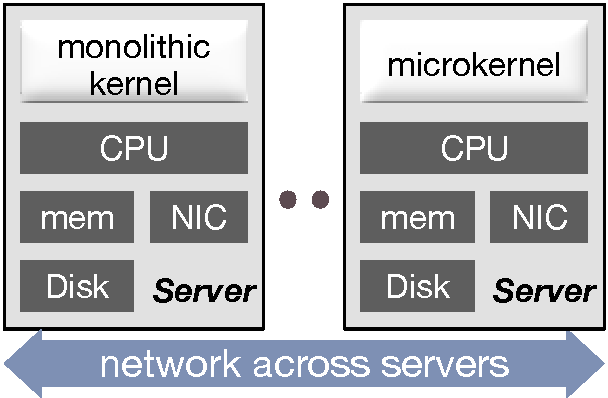
\includegraphics[width=1.7in]{lego/Figures/monolithic-arch.pdf}}
\caption[Monolithic OS.]{OSes Designed for Monolithic Servers.}
\label{fig-monolithic}
\end{center}
\end{subfigure}
\begin{minipage}{0.05in}
\hspace{0.05in}
\end{minipage}
\begin{subfigure}{1.8in}
\begin{center}
\centerline{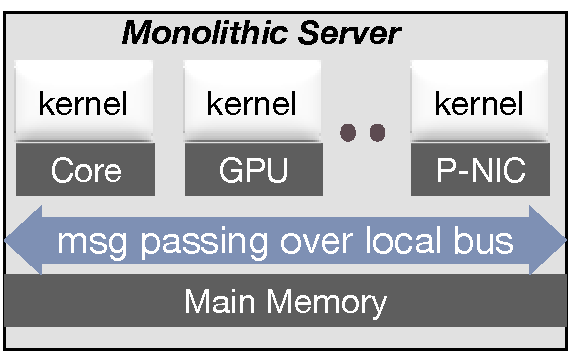
\includegraphics[width=1.8in]{lego/Figures/multikernel-arch.pdf}}
\caption[Multikernel Architecture.]{Multi-kernel Architecture. \small{P-NIC: programmable NIC.}}
\label{fig-multikernel}
\end{center}
\end{subfigure}
\begin{minipage}{0.05in}
\hspace{0.05in}
\end{minipage}
\begin{subfigure}{2.5in}
\begin{center}
\centerline{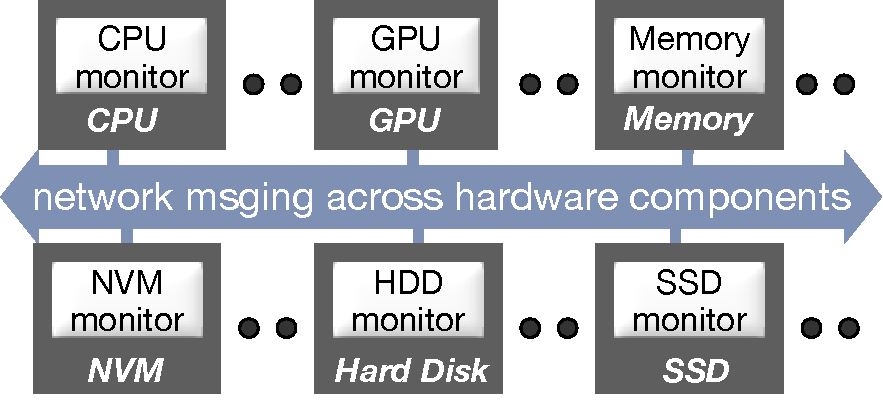
\includegraphics[width=2.6in]{lego/Figures/lego-arch.pdf}}
\caption[Splitkernel Architecture.]{Splitkernel Architecture.}
\label{fig-splitkernel}
\end{center}
\end{subfigure}
\caption[Operating System Architecture.]{Operating System Architecture.}
\end{figure*}
}

We propose {\em \splitkernel}, a new OS architecture for hardware resource disaggregation (Figure~\ref{fig-architecture}).
The basic idea is simple: \textit{When hardware is disaggregated, the OS should be also}.  
A \splitkernel\ breaks traditional operating system functionalities into loosely-coupled {\em \microos{}s},
each running at and managing a hardware component.
Monitors in a \splitkernel\ can be heterogeneous and can be added, removed, 
and restarted dynamically without affecting the rest of the system.
Each \splitkernel\ \microos\ operates locally for its own functionality and
only communicates with other \microos{}s when there is a need to access resources there.
There are only two global tasks in a \splitkernel: 
orchestrating resource allocation across components 
and handling component failure.


We choose not to support coherence across different components in a \splitkernel.
A \splitkernel\ can use any general network to connect its hardware components.
All \microos{}s in a \splitkernel\ communicate with each other via {\em network messaging} only.
With our targeted scale, explicit message passing is much more efficient in network bandwidth consumption 
than the alternative of implicitly maintaining cross-component coherence.

Following the \splitkernel\ model, 
we built \lego, the {\em first} OS designed for hardware resource disaggregation.
\lego\ is a distributed OS that appears to applications as a set of virtual servers (called {\em \vnode{}s}).
A \vnode\ can run on multiple processor, memory, and storage components
and one component can host resources for multiple \vnode{}s.
\lego\ cleanly separates OS functionalities into %{\em micro OS services},
three types of {\em \microos{}s},
process \microos, memory \microos, and storage \microos. %to manage processes, memory, and storage data.
\lego\ \microos{}s share no or minimal states
and use a customized RDMA-based network stack to communicate with each other.

The biggest challenge and our focus in building \lego\ is the separation of processor and memory and their management.
Modern processors and OSes assume all hardware memory units including main memory, page tables, and TLB are local.
Simply moving all memory hardware and memory management software to across the network will not work.

Based on application properties and hardware trends, 
we propose a hardware plus software solution that cleanly separates processor and memory functionalities,
while meeting application performance requirements.
\lego\ moves all memory hardware units to the disaggregated memory components
and organizes all levels of processor caches as virtual caches that are accessed using virtual memory addresses. 
To improve performance, \lego\ uses a small amount (\eg, 4\GB) of DRAM
organized as a virtual cache below current last-level cache.

\lego\ process \microos\ manages application processes and the extended DRAM-cache.
Memory \microos\ manages all virtual and physical memory space allocation and address mappings. 
\lego\ uses a novel two-level distributed virtual memory space management mechanism,
which ensures efficient foreground memory accesses and balances load and space utilization at allocation time.
Finally, \lego\ uses a space- and performance-efficient memory replication scheme to handle memory failure.

We implemented \lego\ on the x86-64 architecture.
\lego\ is fully backward compatible with Linux ABIs
by supporting common Linux system call APIs.
To evaluate \lego, we emulate disaggregated hardware components using commodity servers.
We evaluated \lego\ with microbenchmarks, the PARSEC benchmarks~\cite{PARSEC}, %Filebench~\cite{Filebench},
and two unmodified datacenter applications, Phoenix~\cite{Ranger07-HPCA}
and TensorFlow~\cite{TensorFlow}.
Our evaluation results show that compared to monolithic Linux servers that can hold all the working sets of these applications,
\lego\ is only 1.3\x\ to 1.7\x\ slower with 25\% of application working set available as DRAM cache at processor components.
Compared to monolithic Linux servers whose main memory size is the same as \lego' DRAM cache size
and which use local SSD/DRAM swapping or network swapping,
\lego' performance is 0.8\x\ to 3.2\x.
% (by 0.84\x\ to 3.0\x) or network swapping (by 0.97\x\ to 3.1\x). 
At the same time, \lego\ largely improves resource packing %by up to XXX\x\
and reduces system mean time to failure. % by 18\% to 49\%.

Overall, this work makes the following contributions:

\begin{itemize}

\vspace{-0.065in}
\item We propose the concept of \splitkernel, a new OS architecture that fits the hardware resource disaggregation architecture.

\vspace{-0.065in}
\item We built \lego, the first OS that runs on and manages a disaggregated hardware cluster.

\vspace{-0.065in}
\item We propose a new hardware architecture to cleanly separate processor and memory hardware functionalities, 
while preserving most of the performance of monolithic server architecture.

\vspace{-0.065in}

\end{itemize}

\lego\ is publicly available at {\small {\em {\url{http://LegoOS.io}}}}.\\

\if 0
The rest of the paper is organized as follows.
\S{}2 motivates hardware resource disaggregation and a new OS for it.
\S{}3 presents the concept of \splitkernel.
We then discuss the detailed design and implementation of \lego\ in \S{}4 and \S{}5.
\S{}6 presents our evaluation results of \lego.
Finally, we cover related works in \S{}7 and conclude in \S{}8.
\fi
